\documentclass[12pt, letterpaper]{article}
\usepackage[margin=.5in]{geometry}
\usepackage{graphicx}
\usepackage{tikz}
\usepackage{adjustbox}

\title{
	GV101 Intro to PolSci\\
	\large{Professor Simon Hix}\\
	\large{Short Answer Questions}\\ {Revision Document}
}
\author{Cedric Tan}
\date{April 2019}


\begin{document}
\maketitle
\abstract{This document covers the 8 topics that could be asked in the short answer section of the GV101 paper. There is a section dedicated to each topic and each section will begin with the definitions related to the subject then go into moderate depth on the relevant material before concluding with a half page summary on the topic. 

Note that this is a collation of readings, lecture notes and further supplementary material that can be found online. All work is not necessarily authentic and has been modified by me to fit my needs for this course}

\newpage
\tableofcontents
\newpage


\section{The Modernisation Theory of Democratisation}

\textbf{Definition:} Classic modernisation theory argues that countries are more likely to become democratic and stay democratic as they develop economically $\rightarrow$ this theory is more prevalent in high-income countries. (Clark, Golder and Golder 2017)

\subsection{Key Ideas}
Modernisation theory argues that all societies pass through the same historical stages of economic development. Those who are not democratic are simply \textbf{labelled as underdeveloped.} Rostow (1960) and Gerschenkron (1962) believed that African, Asian and Latin American countries were simply underdeveloped versions of countries in Europe.

These 'primitive' countries were characterised by large agricultural sectors and small industrial and service sectors. Eventually these countries are supposed to modernise by expanding their industrial and service sectors while reducing their emphasis on the level of agriculture.

\subsection{The Political Science Approach}
Helmed by Lipset (1959, 1960), modern societies, he says, need an appropriate type of government. Przeworski (1998, 2000) states that dictatorships and other types of government are replaced by democracies because:
\begin{itemize}
	\item Social structure becomes more complex
	\item New groups emerge and organise along various lines
	\item Labour requires active cooperation by employees hence the system can no longer be \textbf{command driven.}
	\item Dictatorships lose control and effectiveness as:
		\begin{itemize}
			\item Technological change endows private information and autonomy
			\item Civil democratic society tends to emerge as a result
		\end{itemize}
\end{itemize}
Hence for Przeworski, modernisation theory highlights the idea that as a country develops economically, they will also democratise due to the plurality of opinions that are formed along with the independence individuals develop with their new information.

Lipset also argues that higher income countries will also tend to maintain their democratic status as:
\begin{itemize}
	\item Sustaining the democracy is done through the people and their interests
	\item Interest in democracy is a main concern for these people and it persists as long as Przeworksi's reasons of diverse social structure remain
\end{itemize}

\subsection{Summary of Modernisation Theory}
Modernisation theory argues that countries are more likely to become democratic and stay democratic as they develop economically. It argues that all societies pass through the same historical stages of economic development.

Przeworski argues that dictatorships and other types of non-democratic governments are replaced by democracies because as these countries develop economically and socially, societal structure becomes more complex. This is seen by new groups emerging and organising along different cleavage lines.

The economic argument is also extended by how labour, requiring active cooperation, can no longer be command driven. Agricultural sectors decline as service sectors expand with the middle class growing as well. Dictatorships lose control and effectiveness as technological change endows private information and autonomy giving individuals a new-found sense of independence leading to a demand for democracy.

Lipset also argues that democracy lasts longer as peoples interests are sustained through democracy and so it is also in their interests to maintain the democratic process. This theory imples that countries with high levels of GDP tend to be democracies and transitions to dictatorship or out of democracy are less likely as wealth increases.

\newpage
\section{The Selectorate Theory for Non-Democratic Regimes}

\textbf{Definition:} Selectorate theory helps to explain why we observe tremendous variation in the economic performance of dictatorships. Rather than categorise governments as either democratic or dictatorial, selectorate theory characterises all governments by their location in a two-dimensional institutional space:
\begin{itemize}
	\item One dimension is the size of the selectorate: those with a say in selecting the leader
	\item The second is the size of the winning coalition: those in the selectorate whose support is essential for the leader to stay in office
\end{itemize}

\begin{center}
	$W = Winning\;Coalition$ and $S = Selectorate$
\end{center}

\subsection{Types of Selectorate and Winning Coalition}
Here are various forms of the relationship between Selectorate and Winning Coalition:
\begin{itemize}
	\item Large W and Large S
		\begin{itemize}
			\item Democracies usually
			\item Incentive to produce public goods
			\item Good government performance
			\item High levels of wealth, efficient governane and low rates of corruption and kleptocracy
		\end{itemize}
	\item Small W and Large S
		\begin{itemize}
			\item Personalist dictatorships and dominant party democracies
			\item Incentives to provide rewards to their relatively small winning coalition to stay in power
			\item Rigged voting hence the large selectorate but small winning coalition
			\item Poor government performance
			\item Low levels of wealth, inefficient governance with high levels of corruption and kleptocracy
		\end{itemize}
	\item Small W and Small S
		\begin{itemize}
			\item Monarchic and military dictatorships
			\item Produces middling government performance
			\item Moderate levels of corruption and kleptocracy
		\end{itemize}
\end{itemize}

The basic assumption of selectorate theory is that all political leaders are motivated by the desire to gain office. The competitive nature of politics forces all leaders to behave in this way. With that in mind, government performance is derivative of the ruling power making their selectorate happy. As shown above, personalistic or dominant party regimes will have lacking performance due to a small W that needs to be appeased. Dictatorships tend to focus on private goods to be given to their W as a result of this. For democracys, who have large Ws, public goods are the focus.

\subsection{Loyalty Norm}
The \textbf{Loyalty Norm} extends the idea of keeping the respective Ws happy. The Loyalty Norm is determined by $W/S$ which is effectively the probability that someone in the selectorate is in the winning coalition. \\

\textbf{Low Probability:}

There is less chance of a member of W defecting as the odds that they could form a new winning coalition is low, hence the loyalty here is high. Strong loyalty norm regimes tend to have a \textbf{greater chance in engaging in corruption and kleptocracy.} The amount to pay W is lower to keep their loyalty. \\

\textbf{High Probability:}

These is a higher chance of a member of W defecting as the odds that they could form a new winning coalition is high, hence the loyalty here is low. Low loyalty norm regimes tend to have a \textbf{lower chance in engaging in corruption and kleptocracy.} The amount required to pay W is higher to keep their loyalty. 

\begin{center}

We can recognise the probabilities by constructing a simple equation:

% insert equation and example from Clark, Golder and Golder
$R_L = Reward\;for\;Loyalty$ ;
$R_D = Reward\;for\;Defecting$ \\
$P_L = Probablity\;of\;Staying$ ;
$P_D = Probability\;of\;Defecting$ \\

\end{center}

\subsection{Size of the Winning Coalition}
The size of W can affect the eocnomic performance heavily through either investment into public or private goods. Leaders \textbf{always prefer to use private goods to satisfy the winning coalition rather than public goods} as it is easier and more effective. However, \textbf{increasing W should lead to more public good production.} This is simply because there is more people to please and public goods, since they are \textbf{non-rivalrous} \textit{(one person's consumption does not hinder another's ability to consume)} and \textbf{non-excludable} \textit{(one cannot prevent another from accessing this good entirely)}, appease everyone. Private goods, on the other hand, can only entertain a few people and so would not be able to maintain W.

\subsection{Summary of Selectorate Theory}
Selectorate theory helps to explain why we observe tremendous variation in the economic performance of dictatorships. Rather than categorise governments as either democratic or dictatorial, selectorate theory characterises all governments by their location in a two-dimensional institutional space. One is the size of the selectorate, those with a say in selecting the leader. The second is the size of the winning coalition, those in the selectorate whose support is essential for the leader to stay in office. The assumption is that all political leaders are motivated by the desire to gain office.

For non-democratic regimes, usually one requires a small winning coalition irrespective of the size of the selectorate. Hence, leaders in non-democratic regimes prefer to use private goods to satisfy their winning coalition as it is cheaper and more direct making it easier to maintain their power. We can measure their ease of maintaining power through the loyalty norm which shows how likely it is for a leader to lose power. It is measured by $W/S$ which is the ratio of the winning coalition to selectorate. The larger S is relative to W, the more loyal the winning coalition is as the probability of being in another winning coalition after defecting is minimal.

Hence, with a small W and small S, selectorate theory would predict moderate levels of corruption and kleptocracy as the probability of forming another W is higher. This leads to middling government performance. With a small W and large S, we would see high levels of corruption and kleptocracy as leaders would keep their coalition loyal through private goods and poor government performance.

\newpage
\section{Differences between Strategic and Expressive Voting}
\textbf{Definitions:}
\begin{itemize}
	\item \textbf{Strategic:} voting to produce an election outcome which is as close as possible to one's policy preferences (which may or may not mean voting for one's preferred party).
	\item \textbf{Expressive or Sincere:} voting on the basis of party attachment, political ideology or social group membership.
\end{itemize}

The two are often the same i.e. expressively voting is usually strategic voting as well. However, the interesting scenario is when one is \textbf{cross-pressured:} where voting one way means not voting the other way, \textbf{when the two styles of voting are mutually exclusive.}

Voters are assumed to be in a spatial model of politics where each voter has preferences about a range of policies. These preferences are \textbf{single peaked} which means that each voter has an \textbf{ideal point} in a single or multi-dimensional policy space.

\subsection{Expressive}
So as we noted before, expressive means:
\begin{itemize}
	\item Identification with a particular social cleavage, group or ideology
	\item People voting in line with this identity whether it be socio-economic class, ethnic or cultural associations
	\item Religion (Tilley 2015) may also have an effect on how one would vote
	\item Voting for whatever party feels \textbf{closest to me.}
\end{itemize}

Hence, voting expressively is pretty self-explanatory. It is because it is closest to your personal preference that you would vote in that way. If you vote purely in terms of expression, strategic voting does not matter whatsoever. When you are cross-pressured, you will choose the party closest to you.

\subsection{Strategic}
And for strategic we see that:
\begin{itemize}
	\item Citizens vote to try to influence the outcome of an election
	\item Overall policy outcomes that they attempt to influence would be closest to their ideal policy of all the likely outcomes
	\item Citizens attempt to influence outcomes whilst maintaining policy preferences close to their true preferences
\end{itemize}

\subsection{Why vote strategically?}
As opposed to expressive voting, the reasons for voting strategically can differ. Not that when we talked about cross-pressure, the expressive voter did not mind. However, for strategic voters, especially for those who support smaller parties, it is a serious problem as smaller party representatives are unlikely to be elected into office so strategic voters need to reconfigure their vote to influence a policy outcome.

There are two main reasons:
\begin{enumerate}
	\item \textbf{Local:} to influence the election outcome in a constituency. If the candidate a person most preferences has no chance of being elected, then vote for the closest candidate in preference from amongst the candidates who have a reasonable chance of winning. Example:
		\begin{itemize}
			\item British Elections
			\item First preference: Liberal Democrat
			\item \% Voting for Lib Dem as first preference: 56\%
			\item Likelihood is that the others split between Labour and Conservative
		\end{itemize}
	\item \textbf{National:} to influence the government formation and policy outcomes. If the party a person most prefers has no choice of influencing government formation or might form a coalition with a party which is further away from a person's preference, then vote for a party which is 'further away' but which will lead to a policy outcome closer to a person's ideal policy. Example:\\
	\begin{center}
		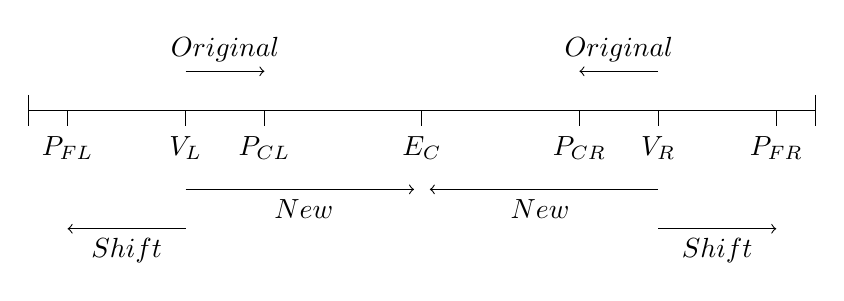
\begin{tikzpicture}
			\draw (-5,0) -- (5,0);
			\draw (-5, .2) -- (-5, -.2);
			\draw (5, .2) -- (5, -.2);
			\coordinate [label=below:$V_L$] (A) at (-3,-.2);
				\draw (-3, 0) -- (-3, -.2);
			\coordinate [label=below:$V_R$] (B) at (3,-.2);
				\draw (3, 0) -- (3, -.2);
			\coordinate [label=below:$E_C$] (C) at (0,-.2);
				\draw (0, 0) -- (0, -.2);
			\coordinate [label=below:$P_{CL}$] (D) at (-2,-.2);
				\draw (-2, 0) -- (-2, -.2);
			\coordinate [label=below:$P_{CR}$] (E) at (2,-.2);
				\draw (2, 0) -- (2, -.2);
			\coordinate [label=below:$P_{FL}$] (F) at (-4.5,-.2);
				\draw (-4.5, 0) -- (-4.5, -.2);
			\coordinate [label=below:$P_{FR}$] (G) at (4.5,-.2);
				\draw (4.5, 0) -- (4.5, -.2);
			\draw [->] (-3, .5) -- (-2, .5);
			\draw [->] (-3, -1) -- (-0.1, -1);
			\draw [->] (-3, -1.5) -- (-4.5, -1.5);
			\coordinate [label=above:${Original}$] (H) at (-2.5, .5);
			\coordinate [label=below:${New}$] (I) at (-1.5, -1);
			\coordinate [label=below:${Shift}$] (J) at (-3.75, -1.5);
			\draw [->] (3, .5) -- (2, .5);
			\draw [->] (3, -1) -- (0.1, -1);
			\draw [->] (3, -1.5) -- (4.5, -1.5);
			\coordinate [label=above:${Original}$] (K) at (2.5, .5);
			\coordinate [label=below:${New}$] (L) at (1.5, -1);
			\coordinate [label=below:${Shift}$] (M) at (3.75, -1.5);
		\end{tikzpicture}
	\end{center}
	
	Hence this result illustrates a shift in voting as a result of a delcared coalition that was further away from the voter's original preferences. Look at $V_L$ which is the left voter and $V_R$ which is the right voter, they would originally vote for the parties on the center-left and center-right respectively. However, after a coalition is announced between those two parties, the new distance from their true preferences is shifted all the way to the middle. They will subsequently shift their vote for the far left and far right parties, although further away, to see some compromise on policy preferences.
\end{enumerate}
It also depends on what type of electoral system is in play. If proportional, it is more likely to see expressive voting. If it's first past the post, there might be more strategic voting.

\subsection{Summary of Expressive and Strategic Voting}
Based on a spatial model of politics, voters each have a preference which is single-peaked. This means that each voter has an ideal point in a single or multi-dimensional policy space.

To vote expressively is to vote based on party attachment, political ideology or social group membership. Individuals who vote expressively vote for the candidate or party closest to their single-peaked preference in the policy space.

To vote strategically is to vote in an attempt to influence the outcome of an election. They attempt to influence policy outcomes which are as close as possible to one's policy preferences but may not be voting for one's preferred party as the preferred party does not have a realistic chance of winning a seat or winning the election.

There are two main reasons to vote strategically: Local and National. The local reason is to influence the election outcome in a constituency. If the candidate an individual most prefers has no chance, then said individual would vote for the closest candidate in preference from amongst the candidates who have a reasonable chance of winning.

The national reason is to influence government formation and policy outcomes. If the party a person most prefers has no chance of getting into government or forms a coalition far away from the individual's preference, then their vote would be directed to a party which lead to an outcome closest to the individual's ideal policy.


\newpage
\section{Down's Theory of Party Competition}
\textbf{Definition:} the simple Downsian model of two-party competition under plurality is generally characterised as predicting party convergence to the policy position espoused by the median voter.

\subsection{Assumption of the Downsian Model}
Below are a list of assumptions that Grofman (2004) thinks Downs has
\begin{enumerate}
	\item The system only has \textbf{two political parties}
	\item Single-round election for any office
	\item The election chooses a single candidate
	\item Elections take place within a single constituency
	\item The election is decided by a \textbf{plurality vote}
	\item Policies can be located a \textbf{single left-right dimension}
	\item \textbf{Candidate policy positions are well defined}
	\item \textbf{Candidate policy positions are accurately estimated by each voter}
	\item Voters look no further than the next decision
	\item Eligible voters go to the polls if the expected benefits of their vote's contribution to the election exceeds costs
	\item Voters care only about which candidate/party will enact policies closest to their preference location. If there are no policy differences, they are equally likely to support each and every candidate
	\item Parties/candidates care only about winning
	\item Parties/candidates look no further than the next election
	\item \textbf{Candidates/parties accurately estimate the policy preferences of voters}, or at minimum,\textbf{ they can identify the location of the median voter} overall or in each party
	\item Candidates are part of a \textbf{unified party team}
\end{enumerate}

\subsection{The Downsian Model}
Assuming that there is a normal distribution of voters, we can model the vote distribution and subsequent convergence as shown below:
\begin{center}
	\begin{tikzpicture}
		\coordinate [label=left:$L$] (A) at (-5, 0);
		\coordinate (B) at (0, 6);
		\coordinate [label=below:$P_A$] (P_A) at (-3, 0);
		\coordinate [label=below:$P_B$] (P_B) at (0, 0);
		\coordinate [label=below:$Split$] (M_P) at (-1.5, 0);
		\coordinate (C) at (0, 0);
		\coordinate [label=right:$R$](D) at (5, 0);
		\draw [thick, dashed] (C) -- (B);
		\draw [thick](A) -- (D);
		\draw (M_P) -- (-1.5 , 5);
		\draw (A) .. controls (0, 7) .. (D);
		\coordinate [label=left:$Vote\;Share$] (Top) at (-5, 6);
		\draw [thick, ->](A) -- (Top);
	\end{tikzpicture}
\end{center}

From the picture above, we can see that the split vote share is given mostly to B as party B is on the median voter line. Hence, the voter base is split at the middle point between $P_A$ and $P_B$. For A to gain more voters, it needs to shift its policy position closer to B so that the split becomes more even. The Downsian model then predict that A will keep shifting until the party reaches the median voter like B. \textbf{It would be the same case if B started at a further right position and they both converged to the median voter. \textit{In game theory this would be called a Nash Equilibrium.}} This would end up looking as you would expect:
\begin{center}
	\begin{tikzpicture}
		\coordinate [label=left:$L$] (A) at (-5, 0);
		\coordinate (B) at (0, 6);
		\coordinate [label=below:$P_A$] (P_A) at (-3, 0);
		\draw [->] (-2.5, -.3) -- (-.9, -.3);
		\coordinate [label=below:$P_{AN}$] (P_AN) at (-0.3, 0);
		\coordinate [label=below:$P_B$] (P_B) at (0.3, 0);
		\coordinate (C) at (0, 0);
		\coordinate [label=right:$R$](D) at (5, 0);
		\draw [thick, dashed] (C) -- (B);
		\draw [thick](A) -- (D);
		\draw (A) .. controls (0, 7) .. (D);
		\coordinate [label=left:$Vote\;Share$] (Top) at (-5, 6);
		\draw [thick, ->] (A) -- (Top);
	\end{tikzpicture}
\end{center}

Thus, both parties have an equal share of the votes as shown by the diagram as $P_A$ shifts to $P_{AN}$.

\subsection{Reasons Why Parties Might Not Converge}
Below are some reasons that parties might not converge which you can be wary of:
\begin{itemize}
	\item Party positions are sticky due to the costs associated with moving
	\item There is threat of competition by flanks. Far right and Far left parties might arise as a result of Downsian convergence
	\item The reality of a multidimensional space, rather than the assumed single one, makes it more difficult to know where to move; it isn't always the median voter!
	\item Low turnout could happen since the fringes are not accounted for. It might be easier to mobilise your base than to capture new voters and persuade them to switch
	\item It is also dependent on how party leaders are chosen, whether it be the average voter, party officials or members which get to choose. This affects whether they are more extreme or moderate
 
\end{itemize}

\subsection{Summary of Downs' Theory of Party Competition}
Downs' theory of party competition predicts party convergence to the policy position espoused by the median voter. He assumes the system has two political parties, the election is decided by a plurality vote and policies are located on a single left-right dimension. Further, candidate policy positions are well defined and estimated accurately by each voter whilst candidates are able to estimate the policy preferences of voters whilst acting as a unified party team.

Thus, based on these assumptions, if we have a normal distribution of voters, Down's theory predicts that parties will keep moving towards the median voter in an attempt to capture more votes to stay in power. This would be shown in the figure below\\\\
\textbf{Assume figure exists but use the one above in notes}
\\\\
From this, we see that initially A has less votes than B but moves towards the median to capture some of B's voters. Then B moves closer to the median to capture back some of A's new voters until we arrive at the equilibrium where the both parties have converged onto the median voter.



\newpage
\section{Olson's Theory of Collective Action}
\textbf{Definitions:} 
\begin{itemize}	
	\item \textbf{Collective Action:} refers to the pursuit of some objective by a group of individuals. Typically the objective is some form of public or private good.
	\item \textbf{Public Good:} a good which is non-excludable, whereby one cannot prevent other people from consuming the good once it is produced, and non-rivalrous, where one's consumption of the good does not affect another's ability to consume the same good.
	\item \textbf{Interest Group:} Any group which seeks to promote a particular policy or set of policies, and to organise to influence politics and policy-makers to achieve this policy.
	\item \textbf{Social Movement:} A large informal group of individuals and/or organisations which aim to promote a particular political or social issue, or promote/resist social change.

\end{itemize}

\subsection{The Logic of Collective Action}
Olson attempts to explain why some groups are more able to mobilise than others and, as a result, why public goods are likely to be undersupplied and private goods oversupplied. He presents us with a \textbf{collective action function} shown below:

\begin{center}
Each individual has a collective action function: \\
$R=(B \times P) - C$ \\
$R$ is the reward for participating in collective action \\
$B$ is the benefit of the good provided by a group \\
$P$ is the probability that the action of the individual makes a difference \\
$C$ is the cost of participation
\end{center}

\begin{center}
\textbf{Example 1: Student Demonstrations} \\
This example is to show the free rider problem we can face in collective action. \\
Taking $R=(B \times P) - C$ \\
$B$ would be cutting tuition fees \\
$P$ would be low as government probably won't change their stance \\
$C$ would be high as you're marching the whole day in the cold! \\
Hence we would have \\
$R=(B \times P) - C$ where $R<0$
\end{center}

Thus there's the free rider problem as individuals have little incentive to join a group which seeks a public good, as they all benefit if the protests are successful $\rightarrow$ there will be students protesting anyway. However, the costs for the individuals exceed the probable benefits.

\begin{center}
\textbf{Example 2: Farm Subsidies} \\
This example shows the power of organised interests \\
For this example, take 20 citizens in society with 4 out of the 20 being farmers. Each citizen \textbf{pays £1 in tax} and each farmer \textbf{receives a £5 subsidy.}

\begin{center}
\begin{tabular}{|c|c|c|c|}

	\hline
	& Tax & Subsidy & Outcome \\
	\hline
	\hline
	Farmers & £1 & £5 & +£4 \\
	\hline
	Individuals & £1 & £0 & -£1 \\
	\hline

\end{tabular}
\end{center}

Taking $R=(B \times P) - C$ \\
$B$ would be cutting tuition fees \\
$P$ would be low as government probably won't change their stance \\
$C$ would be high as you're marching the whole day in the cold! \\
Hence we would have \\
$R=(B \times P) - C$ where $R<0$
\end{center}

Each farmer has an incentive to organise to maintain subsidies while each taxpayer and consumer has no incentive to stop them. This is because farmers represent a concentrated interest seeking a \textbf{private good} while taxpayers represent a diffuse interest, \textbf{they are not aligned unless the tax is insanely high!} Hence farmers mobilise and more likely to get what they want.

\subsection{Diffused and Concentrated Interest}
The difference between the two types of demonstrations can be distilled into the idea of a diffused versus concentrated interest. Depending on the size of groups, smaller groups with are more likely to mobilise due to the concentrated interest that they would naturally share

\subsection{Coordination}
Large groups and small groups also have an affect on coordination and how successful groups can be. If you have a large group, the cost of coordination is much higher whilst for a small group, the costs of coordination are much lower and is simply easier to coordinate.

\subsection{Summary of Collective Action}
Olson's logic of collective action attempts to explain the pursuit of some objective by a group of individuals and why some groups tend to succeed in mobilising more than others. Collective action is usually concerned with the provision of public goods which are non-rivalrous and non-excludable and private goods which are rivalrous and excludable.

Each individual has a collective action function which helps them decide on whether or not they would benefit from collectively acting. This function is $R = (B \times P) - C$ where R is reward for the individual, B is the benefit of the good, P is the probability of attaining the good and C is the cost.

When the good pursued is a public good, there is a free-rider problem. Since the good is non-rivalrous and non-excludable, if the good is successfully obtained, everyone can benefit. Thus the incentive to collective act is low as you would reap the benefits irrespective knowing that your individual contribution would not increase the probability of success by much.
	
When the good pursued is a private good, there is no-free rider problem and the concentrated interest would make it easier for people to mobilise in an attempt to get that good.
	
Further, if the group pursuing a good is small, interest is concentrated making it easier to mobilise and collectively act. If the group is large, interest is diffused making it harder for people to collectively act and mobilise for a good.
	
Hence, interest groups which are small and have a concentrated interest for private goods are more likely to succeed in collective action than groups who are large looking to obtain a public good.


\newpage
\section{Tsbelis' Theory of Veto Players and Agenda Setters}
\textbf{Definitions:}
\begin{itemize}
	\item \textbf{Veto Players:} actors whose agreement is required for a change of the status quo, they have the right to block a proposal e.g. the median member of parliament
	\item \textbf{Agenda Setters:} the right or ability to make a proposal or influence the importance placed on the topics of the public agenda e.g. the government
\end{itemize}

\subsection{Tsebelis Overview}
His view is based on the political system as the means for collective decisionmaking. Consequently, all actors in the system, whether they be voters, representatives or political parties, care about policy outcomes, either directly or indirectly $\rightarrow$ either because they have preferences over outcomes or because other things they like depend on policy outcomes. It attempts to predict \textbf{the likelihood of policy change.}

Policy outcomes are the result of two factors:
\begin{itemize}
	\item The preferences of the actors involved
	\item Prevailing institutions in place
\end{itemize}
More importantly, understanding where the status quo is can affect the stability of policy.

Tsebelis believes that all political institutions are translated into a series of veto-players and agenda-setters. The number and location of veto players affects policy stability, or \textbf{how difficult it is to change the status quo.}

Further, the sequence in which veto players make their decisions affects the influence that these veto players have in the decisionmaking process. If you're an individual veto-player or in a collective group of veto-players, your decisionmaking process will also differ.

\subsection{Individual Veto Players}
We will focus on individual veto players and how they affect policy in simple Euclidean spatial models.

He has two main propositions:
\begin{itemize}
	\item \textbf{More Veto Players $\rightarrow$ Less Policy Change}
	
	Examples include: coalition governments, presidential systems, bicameralism, supreme court, central bank
	\item \textbf{Bigger Policy Distance between Veto Players $\rightarrow$ Less Policy Change}
	
	Examples include: Coalition between two ideologically similar vs between two ideologically different
\end{itemize}

It follows that a change in the status quo requires a unanimous decision of all veto players. 

If veto players are generated by the constitution, they are called \textbf{institutional veto players.} For example, the US Constitution specifies that legislation, to be enacted, requires the approval of the president, House of Representatives and the senate. All three parts of are seen to be veto players.

If veto players are generated by the political game, they are called \textbf{partisan veto players.} For example, it may be that inside the House of Representatives, different majorities exist, the majority party is the real (partisan) veto player even though the house itself is an institutional veto player.\\\\
Each individual veto player is represented by his/her ideal point in an \textit{n-dimensional} policy space. In addition, each veto player has \textit{circular indifference curves}, indifferent between alternatives that have the same distance from his ideal point.
Two more concepts are identified by Tsebelis:
\begin{itemize}
	\item \textbf{Winset of the Status Quo:} the set of policies that would beat the status quo in a pair-wise contest under whatever voting rules are being employed i.e. replace existing policy
	\item \textbf{Core:} the set of points with empty winset i.e. the points that cannot be defeated by any other point if we apply the decisionmaking rule. For example, the \textit{unanimity core} refers to the set of points that cannot be defeated if the decision is unanimous.
\end{itemize}
Thus, depending on these concepts and their relative significance or size, policy stability is affected. Policy stability is the difficult of effecting significant change in the status quo. If the winset is small, policy is more stable as there is less room to change. If the winset is large, policy tends to be more flexible as the area of indifference between the veto players are larger:
\begin{itemize}
	\item If the winset of the status quo exists, its size decreases or remains the same with the addition of new veto players.
	\item If there is a unanimity core, its size increases or remains the same with the addition of new veto players.

\end{itemize}

\textbf{Hence, the addition of a new veto player increases policy stability or leaves it the same.} Through Tsebelis' theory, we can see how much consesus and how many constraints we have and need on an agenda setter.

\subsection{Operationalising the Theory}
Below are examples of operationalising the theory.
\subsubsection{Majoritarian Goverment: Dictatorship of the Majority Party}
\textbf{Assumptions:}
\begin{itemize}
	\item $A$, $B$ and $C$ are in the Left Party and $D$ and $E$ are in the Right Party
	\item $B$ is the leader of the Left Party $\rightarrow$ \textbf{$B$ is the agenda setter}
	\item Following these, if there is party cohesion, B is the dictator
\end{itemize}

\begin{center}
\begin{tikzpicture}
\coordinate [label=left:$Left$] (Left) at (-5,0);
\coordinate [label=right:$Right$] (Right) at (5,0);
\coordinate [label=below:$A_L$] (A) at (-3.5,0);
\coordinate [label=below:$B_L$] (B) at (-2,0);
\coordinate [label=below:$C_L$] (C) at (0,0);
\coordinate [label=below:$D_R$] (D) at (1,0);
\coordinate [label=below:$E_R$] (E) at (3,0);
\coordinate [label=above:$SQ$] (SQ) at (2, 1);
\coordinate [label=above:$X$] (X) at (-2, 1);
\draw [->] (SQ) -- (2, 0);
\draw [->] (X) -- (B);
\draw (Left) -- (Right);

% Draw in status quo with chosen policy X

\end{tikzpicture}
\end{center}
This is because $A$, $B$ and $C$ control the majority in the government and any agenda put through by the agenda setter, $B$, would be supported by the cohesive party. This is even if the status quo is as far away as it is.
\subsubsection{Consensus Government: Compromise but Possible Gridlock}
\textbf{Assumptions:}
\begin{itemize}
	\item $A$ and $B$ are in the Left Party, $C$ is in the Center Party while $D$ and $E$ are in the Right Party
	\item The Left Party and Center Party are in coalition
	\item $B$ is the Prime Minister $\rightarrow$ \textbf{$B$ is the agenda setter}
	\item B has to make a compromise proposal because \textbf{C is a veto player}
\end{itemize}
\begin{center}
\begin{tikzpicture}
\coordinate [label=left:$Left$] (Left) at (-5,0);
\coordinate [label=right:$Right$] (Right) at (5,0);
\coordinate [label=below:$A_L$] (A) at (-3.5,0);
\coordinate [label=below:$B_L$] (B) at (-2,0);
\coordinate [label=below:$C_C$] (C) at (0,0);
\coordinate [label=below:$D_R$] (D) at (1,0);
\coordinate [label=below:$E_R$] (E) at (3,0);
\coordinate [label=above:$SQ$] (SQ) at (2, 1);
\coordinate [label=above:$X$] (X) at (-2, 1);
\draw [thick, <->] (-2, -.7) -- (2, -.7);
\draw [->] (SQ) -- (2, 0);
\draw [->] (X) -- (-2, 0);
\draw (Left) -- (Right);

% Draw in status quo with chosen policy X and winset from C equi-distant both sides to SQ


\end{tikzpicture}
\end{center}
Now with a veto player, there is a winset which is the set of policies that the veto player, $C$, prefers to the status quo. This is shown by the double-headed arrow interval between $SQ$ and $X$. If $B$ proposes anything in this interval, $C$ prefers it to $SQ$ and is likely to agree with B to support the coalition.\\

However, if $SQ$ is in between $B$ and $C$, there is likely to be gridlock. This is because $B$ wants policy to move towards $B$ while $C$ wants policy to move towards $C$. We can show this \textbf{gridlock interval} in the illustration below:
\begin{center}
\begin{tikzpicture}
\coordinate [label=left:$Left$] (Left) at (-5,0);
\coordinate [label=right:$Right$] (Right) at (5,0);
\coordinate [label=below:$A_L$] (A) at (-3.5,0);
\coordinate [label=below:$B_L$] (B) at (-2,0);
\coordinate [label=below:$C_C$] (C) at (0,0);
\coordinate [label=below:$D_R$] (D) at (1,0);
\coordinate [label=below:$E_R$] (E) at (3,0);
\coordinate [label=above:$SQ$] (SQ) at (-1, 1);
\coordinate [label=above:$X$] (X) at (-2, 1);
\draw [thick, <->] (-2, -.7) -- (0, -.7);
\draw [->] (SQ) -- (-1, 0);
\draw [->] (X) -- (-2, 0);
\draw (Left) -- (Right);

% Draw in status quo with chosen policy X and winset from C equi-distant both sides to SQ


\end{tikzpicture}
\end{center}
Simply, a proposal of a new policy $X$, by $B$ would be immediately vetoed but $C$ as it is further away from $C$ in the current status quo. The whole interval presents gridlock assuming that the parties are looking to get policy closest to their preference point.

This gridlock interval changes with ideological distance within coalitions and even opposing parties. The USA, with their parties now so far apart, shows the massive gridlock that they have in their system. Due to this, the amount of policy that can be passed is minimal.
\begin{center}
Tsebelis states: If an exogenous shock occurs, a government with many veto players with big ideological distances among them cannot handle the situation and cannot agree on the necessary policies. (2002 p.185)
\end{center}

\subsection{Summary of Veto Players}
Tsebelis' veto player theory sees the political system as a means for collective decision-making for policy away from the status quo, Tsebelis attempts to predict the likelihood of policy change. His theory is centered around veto-players: actors whose agreement is required for a change of the status-quo as they have the right to block a proposal and agenda setters: actors who have the right or ability to make a proposal or influence the importance placed on the topics of the public agenda.

Tsebelis outlines two key concepts: the winset of the status-quo, which is the set of policies that would beat the status-quo in a pair-wise contest under whatever voting rules are being employed, and the core or gridlock interval, which is the points that cannot be defeated by any other point.

Further, two predictions are made:
\begin{enumerate}
	\item More veto players leads to less policy change
	\item Bigger policy distances between veto players leads to less policy change
\end{enumerate}

This is because when more veto players are added, the winset of the status quo either decreases in size of stays the same. If it decreases in size, then the likelihood of the status-quo changing also decreases. If it does not decrease in size, then the likelihood is as before. Further, the gridlock interval either increases or stays the same with additional veto players increasing policy stability.

If there are bigger policy distances between veto players, less policy change occurs as veto players are unlikely to change their policy due to their inability to agree on necessary compromises that might be needed for the status-quo to change. Further, it is likely that the gridlock interval would be increased in size as well.

Hence, veto-player theory allows us to recognise the probability of policy change or policy stability within a political system. This is based on the amount of people that can stop policy from changing or happening and how ideologically far apart these people are.

\newpage
\section{Office vs Policy Seeking Theories of Coalitions}
\textbf{Definitions:}
\begin{itemize}
	\item \textbf{Office Seeking Theory (Riker 1962):} parties, when negotiating, will try to maximise the number of cabinet seats they can achieve, only \textit{minimum winning coalitions} should form as this minimises the amount of cabinet seats that have to be shared between coalition partners
	\item \textbf{Policy Seeking Theory (Axelrod 1970):} parties will try to maximise their influence over policy outcomes, only \textit{connected coalitions} should form between parties that are next to each other on a policy scale, as this minimises the likely policy disagreements between parties
\end{itemize}
\textbf{Note that these two things are not mutually exclusive and it is entirely possible to find minimum-connected-winning coalitions!}

\subsection{Office Seeking Theory}
The idea of the office seeking theory is to maximise the seats in office that you will take. This means that you will attempt to form a coalition that minimises the amount of portfolios that you need to distribute outside your own party. This comes from \textbf{Gamson's Law:}
\begin{center}
	\textbf{Gamson's Law} states that cabinet portfolios will be distributed among government parties in strict proportion to the number of seats that each party contributes to the government's legislative seat total i.e. the amount of seats your party has should proportionally translate to the amount of portfolios.
\end{center}
Thus the desire to maximise seats leads to the formation of a \textbf{minimal winning coalition (MWC).} This is when there is \textbf{just enough parties and no more} required to control a legislative majority, if one pulls out, the coalition does not have any control over the majority. A \textbf{least minimal winning coalition} is a MWC with the lowest number of surplus seats. For example, if we have:
\begin{center}
\begin{tabular}{|c|c|c|}

\hline
Party & \% Seats & Party Position\\
\hline
Party 1 & 45\% & Far Right\\
\hline
Party 2 & 7\% & Far Left\\
\hline
Party 3 & 4\% & Center\\
\hline
Party 4 & 2\% & Center Left\\
\hline
Party 5 & 36\% & Center Right\\
\hline
Party 6 & 6\% & Moderate Right\\
\hline

\end{tabular}
\end{center}

In this, on the assumption that we need 51\% to control a majority, we can find a few coalitions such as Party 1 and Party 2 which gains 52\% of the seats, Party 2, 4, 5 and 6 which gives us 51\% and Party 1, 3 and 4 which also gives us 51\%. The coalitions which give us 51\% of the seat share are \textbf{least minimal winning coalitions.} The second assumption, after choosing the minimal winning coalition is that the parties would choose the least minimal so that the seat share is less distributed among the coalitions. Thus this is what we can conclude from a \textbf{purely office seeking world.} In this world, party position does not matter, as shown above.

\subsection{Policy Seeking Theory}
The idea of policy seeking theory is to create coalitions based on policy concessions. This is because parties seeking to be in power are aiming to implement their own policies that they are advocating for. They no longer simply seek office. Hence, when making concessions on policy, the positions of parties matter greatly. This means that you want to form governments with parties close to you in policy space. 

Political scientists often refer to this type of coalition as a \textbf{connected coalition} where members of the coalition are next to one another in the policy space. If we take a political spectrum as illustrated below:
\begin{center}
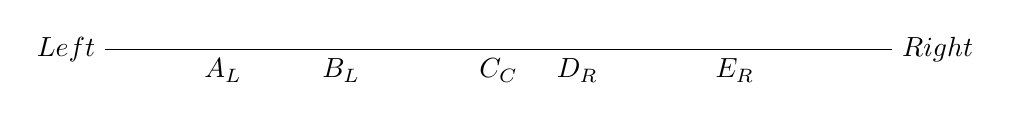
\begin{tikzpicture}
\coordinate [label=left:$Left$] (Left) at (-5,0);
\coordinate [label=right:$Right$] (Right) at (5,0);
\coordinate [label=below:$A_L$] (A) at (-3.5,0);
\coordinate [label=below:$B_L$] (B) at (-2,0);
\coordinate [label=below:$C_C$] (C) at (0,0);
\coordinate [label=below:$D_R$] (D) at (1,0);
\coordinate [label=below:$E_R$] (E) at (3,0);
\draw (Left) -- (Right);

% Draw in status quo with chosen policy X and winset from C equi-distant both sides to SQ

\end{tikzpicture}
\end{center}

We can see that Parties such as $A$ and $B$, if they control the majority of the vote, can form a connected coalition. However, if parties $A$ and $E$ were to form a coalition, this would not be connected since they are on opposite sides of the spectrum.

A second implication of the purely polic--seeking logic is that you will choose the connected least minimal winning coalition. This is to reduce the amount of policy concessions that you'd have to have to be in power. This means that we take our logic from the office seeking theory and combine it with policy seeking incentives to arrive at \textbf{the connected least minimal winning coalition.}

\subsection{Summary of Office vs Policy Seeking Theories}
Riker (1962) through his office seeking theory states that parties, when negotiating, will try to maximise the number of cabinet seats they can achieve when getting into power. Hence, only minimum winning coalitions should form as this minimises the amount of cabinet seats that have to be shared between coalition partners. A minimum winning coalition is a coalition that has just enough parties and no more, such that removing any one party would lose the majority. A least minimum winning coalition would be a coalition that minimises the surplus of seats over the majority.

This comes from Gamson's Law which states that cabinet portfolios will be distributed among government parties in strict proportion to the number of seats that each party contributes to the winning coalition. Hence, behaviour described by Riker would only exist in a purely office seeking world.

Axelrod (1970) though his policy seeking theory states that parties will try to maximise their influence over policy outcomes. Hence, only connected coalitions should form between parties that are next to each other on a policy scale. This theory is based on minimising policy concessions to get into power as parties are seeking to implement their own policies in addition to seeking office.

These two theories are not mutually exclusive. Hence, combining office seeking theory and policy seeking theory, we can predict parties forming connected least minimal winning coalitions which minimises the surplus of seats to gain a majority whilst being ideologically close to their coalition partners.

This occurred in Germany in 2009 where the CDU formed a coalition with the FDP as it was a smaller party than the SDP but still ideologically close.

\newpage
\section{Principal-Agent Theory of Independent Institutions}
\textbf{Definitions:}
\begin{itemize}
	\item \textbf{Principal:} the delegator, usually the politicians who outsource certain tasks to institutions
	\item \textbf{Agent:} the delegatee, usually the institution who acts on behalf of the politicians
	\item \textbf{Moral Hazard:} occurs when the agent has the opportunity to take agents that are hidden from the principal
	\item \textbf{Adverse Selection:} occurs when the agent has attributes that are hidden from the principal
	\item \textbf{Ex Ante Mechanism:} helps principals learn about their agents before these agents are chosen e.g. education and experience filtering
	\item \textbf{Ex Post Mechanism:} helps principals learn about agents actions after they have occurred. This is usually performance and how well they have conformed to the principal's ideas
	\begin{itemize}
		\item In a \textbf{Fire Alarm} system, the principal relies on iformation from others to learn about their agent.
		\item In a \textbf{Police Patrol} system, the principal monitors their agents actions
	\end{itemize}	 
\end{itemize}
This theory was first used in the study of US Government from a political science perspective where we saw legislature vs the executive. However, it is now used increasingly everywhere through analysis of parliamentary government, EU politics, international organisations etc.

\subsection{Principal Agent (PA) Theory Insights}
The main insights of this theory are as follows:
\begin{itemize}
	\item Explains why principals delegate to independent agents
	\item Explains why agents do not do as they are told i.e. \textbf{policy drift}
	\item Explains how policy drift can be reduced
\end{itemize}
These will be explained in the following subsections.
\subsection{Why Delegate?}
Here are some reasons why:
\begin{itemize}
	\item To \textbf{protect particular policies from short-term change} by a particular political majority
	\item To \textbf{establish a credible commitment} to a particular policy
	\item To \textbf{reduce workload} and enhance efficiency in decision-making
	\item To increase \textbf{the use of experts in policy making}
	\item To avoid taking blame for unpopular policies i.e. \textbf{blame shifting}
	\item To produce \textbf{stable and predictable policies}
\end{itemize}
In terms of Courts and Central Banks, here are some reasons to delegate:
\begin{center}
\begin{tabular}{c|c}
Courts & Central Banks\\
\hline
Protect Human Rights & Time inconsistent preferences\\
Complete legislative contracts & End political business cycle\\
Control other agencies & Lock-in stable macro-economic environment\\
\hline
\end{tabular}
\end{center}
Hence, delegation to these institutions ensure more stability in policy over time across the board whilst also providing credibility to their agreements

\subsection{Policy Drift}
Yet, despite all the delegation, policy drift, which is the difference between what the principal desires and what the agent actually does, can still occur. This is even with our mechanisms of selection. Here are reasons why:\\\\
\textbf{The Cause:} the agent does not have the same \textit{policy preferences} as the principal.\\\\
\textbf{Causes of Differences in Preferences:}
\begin{itemize}
	\item Appointment procedure $\rightarrow$ biased preferences of the agent such as judges appointing judges
	\item Specialised knowledge of agents that principals do not have
	\item Institutional/budgetary interests of agency that might not be aligned with the principals ideas
	\item Capture of agent by private interests $\rightarrow$ lobbying, for example, by big banks for the central bank to be \textbf{hawkish} or \textbf{dovish} in certain periods of the economic cycle
\end{itemize}
In terms of Courts and Central banks, here are some reasons for policy drift:
\begin{center}
\begin{adjustbox}{width=.85\textwidth}
\begin{tabular}{c|c}
Courts & Central Banks\\
\hline
Judges tend to be & Central bankers are naturally hawks \\ 
old, rich, white men & $\rightarrow$ against inflation \\
Liberal legal training  & Epistemic community of \\ $\rightarrow$ protect individuals vs the state & neoclassical economists\\
Asymmetric access to courts & Closer connection to \\  $\rightarrow$ they favour the rich and powerful & financial institutions\\
\hline
\end{tabular}
\end{adjustbox}
\end{center}

\subsection{Controlling Policy Drift}
Here are a few methods of controlling policy drift:
\begin{itemize}
	\item Appoint new agents
	\item Restrict bugdet of an agency
	\item Write detailed legislation \textbf{to limit discretion of agents}
	\item Parliamentary scrutiny of agency actions
	\item Delegate to courts to constrain agency e.g. \textbf{competition authority}
	\item New laws e.g. \textbf{revise agency mandate}
\end{itemize}
In the context of Courts and Central banks:
\begin{center}
\begin{adjustbox}{width=.85\textwidth}
\begin{tabular}{c|c}

Courts & Central Banks\\
\hline
Politicised Supreme Courts & Partisan Appointment of Governors\\
Partisan Appointment of Judges & Appointment of non-economists to boards\\
Creation of Special Courts & Separation of mandate $\rightarrow$\\ 
& politicians set inflation target, banks the interest\\
\hline

\end{tabular}
\end{adjustbox}
\end{center}

\subsection{Summary of Principal-Agent Theory}
The Principal Agent Theory provides a mechanism to explain why principals delegate to independent agents, why these agents drift and how this drift can be minimised.

The principal is the delegator and they are usually politicians who outsource certain tasks while the agent is the delegatee, usually an institution such as a central bank, who acts on behalf of these politicians.

The reasons for delegating include: protecting particular policies from short-term change, establishing a credible commitment to a particular policy, to reduce workload for themselves, to use expert information, to avoid taking blame for something deemed unpopular and to produce stable and predictable policy.

Agents, however, might drift as a result of biased preferences they might have which are not aligned with the politician, specialised knowledge that might drive them to do things differently, budgetary or institutional interests that might get in the way or even capture by private institutions such as big banks and lobbyists.

Hence, to control policy drift, one can use ex-ante or ex-post mechanisms such as screening agents and writing legislation to limit their discretion, or punishing them by appointing new agents in their place whilst restricting their budget.

\newpage
\section{Structuring the Answer}
Below is a short guide on how to structure the answer for the exam. Remember that you have to respond directly to the question and so it is entirely dependent on what question you have to show what material you understand. 

For example, for Down's theory of party competition, if the question does not explicitly ask for \textbf{why some parties may not converge,} you do not need to explain this reasoning in your answer.\\\\
\textbf{A good structure is as follows:}
\begin{enumerate}
	\item Introduce what the theory aims to do in an introductory sentence which effectively gives a brief overview
	\item Go into further depth on the theory and what it does, the model or the assumptions associated with the theory
	\item Summarise the theory with a sentence to finish stating that based on these ideas X does Y
\end{enumerate}
Below we will give some examples on structure. Afterwards, refer back to the summaries to memorise the most relevant information, formatted like an answer, then apply said information given the context of the question.

\begin{center}
	\fbox{\begin{minipage}{.9\textwidth}
	\textbf{Explain Olson's (1965) logic of collective action}\\\\
	Olson's logic of collective action attempts to explain the pursuit of some objective by a group of individuals and why some groups tend to succeed in mobilising more than others. Collective action is usually concerned with the provision of public goods which are non-rivalrous and non-excludable and private goods which are rivalrous and excludable.\\
	
	Each individual has a collective action function which helps them decide on whether or not they would benefit from collectively acting. This function is $R = (B \times P) - C$ where R is reward for the individual, B is the benefit of the good, P is the probability of attaining the good and C is the cost.\\
	
	When the good pursued is a public good, there is a free-rider problem. Since the good is non-rivalrous and non-excludable, if the good is successfully obtained, everyone can benefit. Thus the incentive to collective act is low as you would reap the benefits irrespective knowing that your individual contribution would not increase the probability of success by much.\\
	
	When the good pursued is a private good, there is no-free rider problem and the concentrated interest would make it easier for people to mobilise in an attempt to get that good.\\
	
	Further, if the group pursuing a good is small, interest is concentrated making it easier to mobilise and collectively act. If the group is large, interest is diffused making it harder for people to collectively act and mobilise for a good.\\
	
	Hence, interest groups which are small and have a concentrated interest for private goods are more likely to succeed in collective action than groups who are large looking to obtain a public good.
	
	\end{minipage}}
\end{center}


\end{document}
